% =====================================================================
%  LAB 02 - SMOOTHING & EDGE DETECTION: MANUAL IMPLEMENTATION vs LIBRARY
%  Layout mirrors a single-column academic-paper style.
%  Compile with pdfLaTeX (Overleaf -> pdfLaTeX). No source code is embedded.
% =====================================================================
\documentclass[a4paper,11pt]{article}

\usepackage[utf8]{inputenc}
\usepackage[T5]{fontenc}            % T5 so Vietnamese author names render
\usepackage[english]{babel}
\usepackage{lmodern}
\usepackage[margin=2.5cm]{geometry}
\usepackage{graphicx}
\usepackage{booktabs}
\usepackage{array}
\usepackage{amsmath}
\usepackage{amssymb}
\usepackage{float}
\usepackage{enumitem}
\usepackage{algorithm}
\usepackage[noend]{algpseudocode}
\usepackage[labelsep=colon,font=small,labelfont=bf]{caption}
\usepackage{hyperref}
\hypersetup{colorlinks=true, linkcolor=blue!55!black, citecolor=blue!55!black,
            urlcolor=blue!55!black}

\renewcommand{\figurename}{Fig.}      % "Fig. 1:" like the sample
\renewcommand{\arraystretch}{1.2}

% Italic run-in paragraph header (e.g. "Task.")
\newcommand{\runin}[1]{\par\medskip\noindent\textit{#1}\hspace{0.4em}\ignorespaces}

\title{\vspace{-1.2cm}\textbf{\large Comparing Image-Processing Methods:}\\[2pt]
\textbf{\large Manual (NumPy) Implementation vs Standard Library (OpenCV)}\\[3pt]
\normalsize\textit{Lab 02 --- Smoothing and Edge Detection}}

\author{
\normalsize Lưu Thị Yến Nhi \quad\quad Hoàng Trọng Vũ\\[2pt]
\normalsize Advanced Computer Vision --- Lab 02\\
\normalsize Student IDs: 25C11014, 25C15028\\
\normalsize \texttt{nina.dsa@sms-vn.com}
}
\date{\today}

\begin{document}
\maketitle

% --------------------------- ABSTRACT --------------------------------
\noindent\textbf{Abstract.}\hspace{0.4em}
This report implements two groups of image-processing operations twice: once
\emph{from scratch} in NumPy and once via OpenCV, then compares the two
pixel-for-pixel. The groups are (i) smoothing (Mean, Gaussian, Median, Bilateral,
Box) and (ii) edge detection (Roberts, Prewitt, Sobel, Scharr, Laplacian, the
Laplacian-/Difference-of-Gaussian, and a full Canny pipeline). Almost every manual
operation is built on a single hand-written primitive --- a 2D correlation that
replicates \texttt{cv2.filter2D} (correlation with \texttt{BORDER\_REFLECT\_101}
padding). Agreement is measured with Mean Absolute Error (MAE) and PSNR on
\texttt{lena.jpg}. Once each manual operator is paired with the \emph{matching}
library call, every \emph{linear} operator agrees \emph{exactly} (MAE $=0$): Mean,
Median, Box, Roberts, Prewitt, Sobel, Scharr, Laplacian, LoG and DoG. Gaussian blur
leaves only $\approx0.006$ MAE from floating-point rounding against
\texttt{cv2.getGaussianKernel}. The two structurally different cases are the
\emph{bilateral filter} ($\approx0.93$ MAE, because OpenCV approximates the range
weight with quantized look-up tables) and \emph{Canny}: its non-linear non-maximum
suppression (NMS) and hysteresis make a bit-exact match impossible, yet the manual
and OpenCV edge maps still agree on $99.5\%$ of pixels. One lesson stands out: a
naive NMS that snaps the gradient angle to $0/45/90/135^\circ$ thins far too
aggressively (it kept only $\approx37\%$ as many edge pixels as OpenCV); switching
to sub-pixel \emph{interpolated} NMS cut the Canny MAE from $4.78$ to $1.22$.

% =====================================================================
\section{Introduction}
% =====================================================================
\runin{Goal.} This report is a \emph{comparative study}: for each operation we
implement it twice --- once manually in NumPy and once with OpenCV --- and quantify
how closely the two agree. The operations span two groups: smoothing (five low-pass
filters) and edge detection (four first-order gradient operators, the second-order
Laplacian, the LoG/DoG blob filters, and the Canny detector). The central question
is not merely ``does it work'' but ``\emph{how exactly does a hand-built method match
its library counterpart, and where it does not, why}''.

\runin{Scope.} Smoothing runs on the RGB \texttt{uint8} image; edge detection runs
on a single intensity channel obtained with the ITU-R BT.601 luminance
$Y=0.299R+0.587G+0.114B$. Almost every operator is built on one primitive, a 2D
\emph{correlation} that matches \texttt{cv2.filter2D}: the kernel is applied as
stored (not flipped) and the border uses \texttt{BORDER\_REFLECT\_101}, i.e.\
NumPy's \texttt{np.pad(\dots,mode="reflect")}. Matching these two conventions is
what lets a from-scratch filter agree with the library to within rounding.

\runin{Core ideas.} The implementation rests on three ideas:
\begin{itemize}[nosep,leftmargin=1.4em]
  \item \textbf{One convolution primitive.} The linear smoothers and the gradient
        operators are all the same operation --- a small kernel correlated with the
        image --- differing only in the kernel. We write it once and reuse it.
  \item \textbf{Separable Gaussian.} The 2D Gaussian kernel is the outer product of
        a 1D kernel with itself, identical to \texttt{cv2.getGaussianKernel}; it
        underlies Gaussian blur, LoG, DoG and the smoothing step of Canny.
  \item \textbf{Non-linear filters as the hard cases.} The median, bilateral and
        Canny filters are \emph{not} a single correlation; they make per-pixel
        decisions, which is exactly where a from-scratch version can drift from a
        library.
\end{itemize}

% =====================================================================
\section{Method}
% =====================================================================

\subsection{The Convolution Primitive}
Every linear filter here is a 2D correlation of the image $I$ with a kernel $K$ of
size $k_h\times k_w$:
\begin{equation}
(I\star K)(y,x)=\sum_{i=0}^{k_h-1}\sum_{j=0}^{k_w-1}
K(i,j)\,I\!\left(y+i-\lfloor k_h/2\rfloor,\ x+j-\lfloor k_w/2\rfloor\right).
\label{eq:corr}
\end{equation}
We implement Eq.~\eqref{eq:corr} \emph{vectorized}, as a sum of shifted, weighted
copies of the reflect-padded image (one term per kernel tap), so there is no Python
pixel loop (Algorithm~\ref{alg:corr}).

\begin{algorithm}[H]
\caption{Manual 2D correlation (matches \texttt{cv2.filter2D})}
\label{alg:corr}
\begin{algorithmic}[1]
\State Pad $I$ by $\lfloor k_h/2\rfloor,\lfloor k_w/2\rfloor$ with BORDER\_REFLECT\_101
\State $O \gets 0$
\For{each kernel tap $(i,j)$ with $K(i,j)\neq0$}
  \State $O \gets O + K(i,j)\cdot(\text{padded image shifted by }(i,j))$
\EndFor
\State \Return $O$
\end{algorithmic}
\end{algorithm}

\subsection{Smoothing Filters}
\runin{Mean / Box.} The mean (and the normalised box) filter is Eq.~\eqref{eq:corr}
with a constant kernel $K=\tfrac{1}{k^2}\mathbf{1}_{k\times k}$ --- a plain
neighbourhood average.

\runin{Gaussian.} A Gaussian blur uses the (separable) Gaussian kernel
\begin{equation}
g(t)=\exp\!\left(-\frac{t^2}{2\sigma^2}\right),\qquad
K = \frac{g\,g^{\!\top}}{\sum g\,g^{\!\top}},
\label{eq:gauss}
\end{equation}
sampled at integer offsets and normalised to sum~1 --- exactly the kernel produced
by \texttt{cv2.getGaussianKernel}.

\runin{Median.} The median filter is \emph{non-linear}: each output pixel is the
median of its $k\times k$ neighbourhood. We stack the $k^2$ shifted windows and
reduce with \texttt{np.median}. Because the median selects an existing sample, there
is no rounding, so the manual result is bit-exact.

\runin{Bilateral.} The bilateral filter is edge-preserving: it averages neighbours
with a weight that combines a spatial Gaussian and a \emph{range} (intensity) Gaussian,
\begin{equation}
O(p)=\frac{1}{W_p}\sum_{q\in\Omega} I(q)\,
\exp\!\Big(\!-\tfrac{\lVert p-q\rVert^2}{2\sigma_s^2}\Big)\,
\exp\!\Big(\!-\tfrac{\lVert I(p)-I(q)\rVert^2}{2\sigma_r^2}\Big),
\label{eq:bilat}
\end{equation}
so pixels across a strong edge get little weight and the edge is preserved while
flat regions are smoothed.

\subsection{Edge Detection: Gradient Operators}
First-order operators estimate the image gradient with two masks (one per axis) and
report the magnitude:
\begin{equation}
G_x = I\star K_x,\quad G_y = I\star K_y,\quad
\lVert\nabla I\rVert=\sqrt{G_x^2+G_y^2}.
\label{eq:grad}
\end{equation}
Roberts uses $2\times2$ diagonal masks; Prewitt, Sobel and Scharr use $3\times3$
masks with increasingly accurate centre weighting:
\begin{equation*}
K_x^{\text{Rob}}\!=\!\begin{bmatrix}1&0\\0&-1\end{bmatrix}\!,\;
K_x^{\text{Pre}}\!=\!\begin{bmatrix}-1&0&1\\-1&0&1\\-1&0&1\end{bmatrix}\!,\;
K_x^{\text{Sob}}\!=\!\begin{bmatrix}-1&0&1\\-2&0&2\\-1&0&1\end{bmatrix}\!,\;
K_x^{\text{Sch}}\!=\!\begin{bmatrix}-3&0&3\\-10&0&10\\-3&0&3\end{bmatrix}\!.
\end{equation*}
\runin{Laplacian, LoG, DoG.} The Laplacian $\nabla^2 I = I\star K^{\text{Lap}}$
(with $K^{\text{Lap}}$ the 4-neighbour mask) is a second-order operator; we display
$\lvert\nabla^2 I\rvert$. Because the Laplacian amplifies noise, it is usually
applied after smoothing --- the \emph{Laplacian of Gaussian} (LoG). The
\emph{Difference of Gaussians} (DoG), $G_{\sigma_1}\!*I - G_{\sigma_2}\!*I$, is a
fast approximation of the LoG. All three are compositions of linear filters, so they
match the library exactly.

\subsection{Edge Detection: the Canny Pipeline}
Canny turns a gradient field into thin, connected edges in five stages
(Algorithm~\ref{alg:canny}). Stages 1--2 reuse the primitives above. Stage~3,
\emph{non-maximum suppression} (NMS), thins ridges to one-pixel width by keeping a
pixel only if its magnitude is a local maximum \emph{along the gradient direction}.
Rather than snapping the direction to $0/45/90/135^\circ$ and comparing the two
adjacent pixels, we \emph{linearly interpolate} the magnitude at the two points
exactly $\pm1$ step along the gradient from the four surrounding neighbours --- the
same sub-pixel comparison OpenCV performs. Stage~4 labels pixels \emph{strong}
($\ge$ high threshold) or \emph{weak} (between the thresholds); stage~5,
\emph{hysteresis}, keeps a weak pixel only if it is 8-connected (transitively) to a
strong one, implemented by repeatedly dilating the strong set into weak neighbours
until it stops growing.

\begin{algorithm}[H]
\caption{Manual Canny edge detector}
\label{alg:canny}
\begin{algorithmic}[1]
\State Smooth: $S \gets I \star K^{\text{Gauss}}$
\State Gradient: $G_x\gets S\star K_x^{\text{Sob}}$, $G_y\gets S\star K_y^{\text{Sob}}$;
       $M\gets\sqrt{G_x^2+G_y^2}$
\State NMS: keep $M(y,x)$ only if it $\ge$ both interpolated neighbours along $\nabla I$
\State Threshold: \textit{strong} $=\{M\ge t_{\text{hi}}\}$, \textit{weak} $=\{t_{\text{lo}}\le M< t_{\text{hi}}\}$
\State Hysteresis: grow \textit{strong} into 8-connected \textit{weak} pixels until stable
\State \Return binary edge map
\end{algorithmic}
\end{algorithm}

% =====================================================================
\section{Results}
% =====================================================================

\subsection{Qualitative Results}
In every figure the \textbf{columns are the method} (Manual vs Library) and the
\textbf{rows are the operations}, so the two implementations sit side by side
(Figures~\ref{fig:smooth}--\ref{fig:edge}).

\begin{figure}[H]
\centering
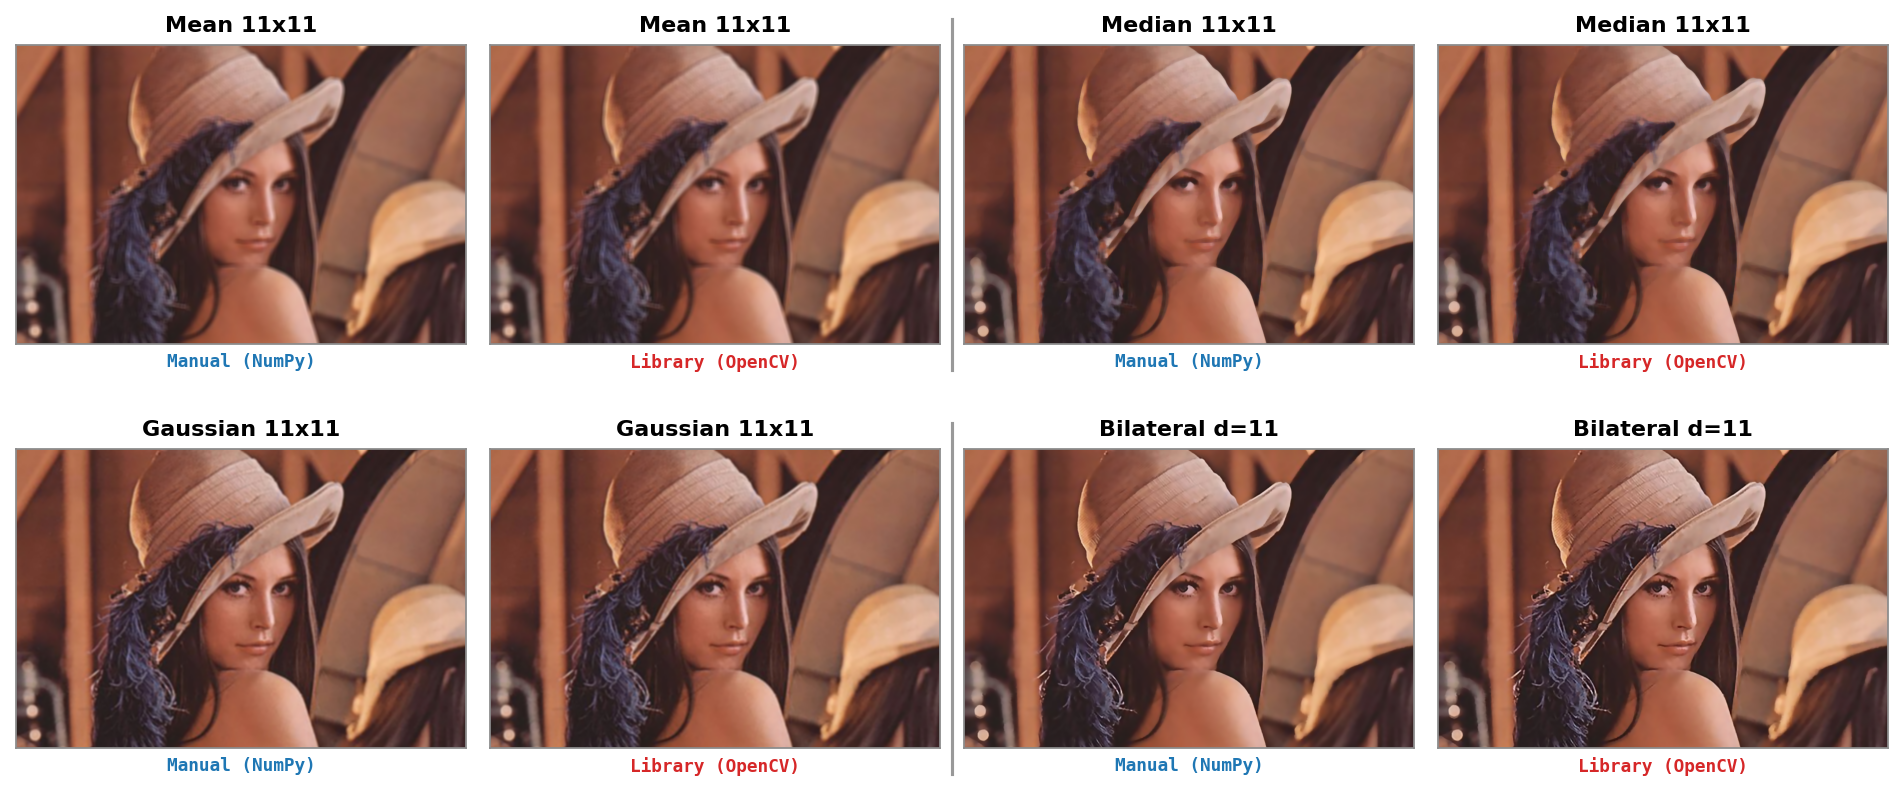
\includegraphics[width=0.52\linewidth]{figures/01_smoothing.png}
\caption{Smoothing (Mean, Gaussian, Median, Bilateral, Box). Each manual filter is
visually indistinguishable from its OpenCV counterpart; the bilateral row keeps the
edges sharp while flattening texture.}
\label{fig:smooth}
\end{figure}

\begin{figure}[H]
\centering
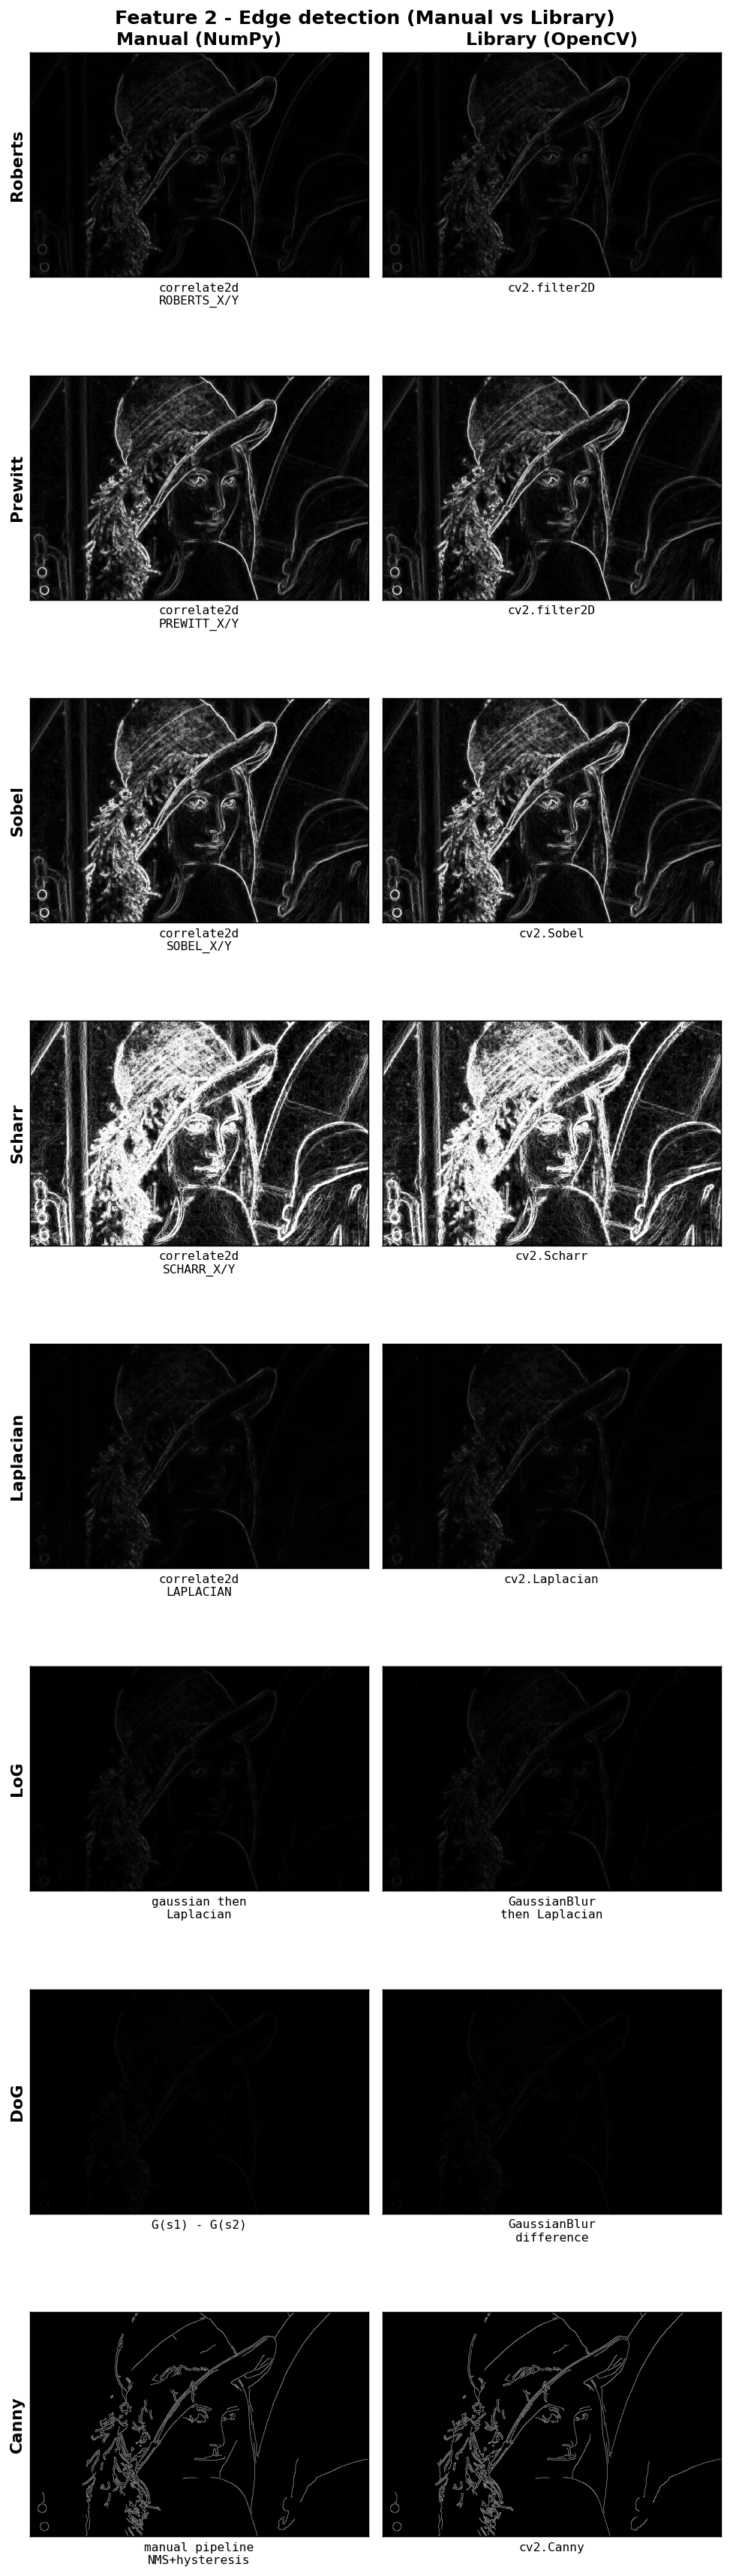
\includegraphics[width=0.52\linewidth]{figures/02_edge_detection.png}
\caption{Edge detection (Roberts, Prewitt, Sobel, Scharr, Laplacian, LoG, DoG,
Canny). Manual and library columns are identical for the linear operators; the Canny
row recovers nearly the same contours as \texttt{cv2.Canny}.}
\label{fig:edge}
\end{figure}

\subsection{Quantitative Comparison}
\label{sec:quant}
Table~\ref{tab:metrics} reports MAE and PSNR between each manual result and its
library counterpart.

\begin{table}[H]
\centering
\caption{Manual vs library agreement on \texttt{lena.jpg}.}
\label{tab:metrics}
\begin{tabular}{l c c p{5.8cm}}
\toprule
\textbf{Feature} & \textbf{MAE} & \textbf{PSNR (dB)} & \textbf{Reason for the difference} \\
\midrule
Mean $5\times5$              & 0.000 & $\infty$ & Identical box kernel \\
Gaussian $5\times5,\sigma{=}1$ & 0.006 & 70.61 & Same kernel; float rounding only \\
Median $5\times5$            & 0.000 & $\infty$ & Exact (median picks a real sample) \\
Bilateral $d{=}5$            & 0.932 & 43.05 & OpenCV uses quantized range LUTs \\
Box $5\times5$               & 0.000 & $\infty$ & Identical to mean \\
Roberts                      & 0.000 & $\infty$ & Identical $2\times2$ kernels \\
Prewitt                      & 0.000 & $\infty$ & Identical (vs \texttt{cv2.filter2D}) \\
Sobel                        & 0.000 & $\infty$ & Identical (vs \texttt{cv2.Sobel}) \\
Scharr                       & 0.000 & $\infty$ & Identical (vs \texttt{cv2.Scharr}) \\
Laplacian                    & 0.000 & $\infty$ & Identical (\texttt{ksize}=1 kernel) \\
LoG                          & 0.000 & $\infty$ & Gaussian + Laplacian (both linear) \\
DoG                          & 0.000 & $\infty$ & Difference of two Gaussian blurs \\
Canny                        & 1.222 & 23.19 & Non-linear NMS/hysteresis; 99.52\% label agreement \\
\bottomrule
\end{tabular}
\end{table}

\runin{Analysis.} With the matching library call, every \emph{linear} operator
agrees exactly: the smoothing box/Gaussian kernels and the gradient masks of
\texttt{cv2.Sobel}/\texttt{cv2.Scharr}/\texttt{cv2.Laplacian} are identical to ours,
and \texttt{BORDER\_REFLECT\_101} padding removes the only other source of
disagreement. Median is also exact, since it selects an actual sample rather than
averaging. Gaussian (and therefore LoG/DoG, when computed in floating point) leaves
at most a $0.006$ MAE residual purely from rounding of the same closed-form kernel.
The two cases that \emph{cannot} match bit-for-bit are non-linear. The bilateral
filter differs by $\approx0.93$ MAE because OpenCV approximates the range-weight
exponential with a quantized look-up table, whereas we evaluate it directly. Canny
differs because NMS and hysteresis are per-pixel decisions where a sub-pixel
difference flips a pixel between edge and non-edge; here two findings are worth
noting. First, the choice of NMS matters: our first version snapped the gradient
direction to the nearest $45^\circ$ and compared the two adjacent pixels, which
thinned far too aggressively, retaining only $6{,}612$ edge pixels against OpenCV's
$17{,}679$ (MAE $4.78$). Replacing it with sub-pixel \emph{interpolated} NMS raised
the count to a comparable level and cut the MAE to $1.22$. Second, even though the
raw gradient magnitudes are essentially identical (manual mean $25.08$ vs OpenCV
$25.15$), the final maps still differ slightly because OpenCV runs hysteresis in
integer arithmetic; the $99.5\%$ pixel agreement confirms the residual is confined
to a thin halo around the contours.

% =====================================================================
\section{Work Assignment and Completion}
% =====================================================================
Per-member effort is broken down in Appendix~\ref{app:effort}.

\begin{table}[H]
\centering
\caption{Members and assigned work.}
\label{tab:members}
\begin{tabular}{c l c p{5.6cm} c}
\toprule
\textbf{No.} & \textbf{Full name} & \textbf{Student ID} & \textbf{Assigned tasks} & \textbf{Share} \\
\midrule
1 & Lưu Thị Yến Nhi & 25C11014 &
  Feature 1 (smoothing filters, shared toolbox); report sections 1, 4. & 50\% \\
2 & Hoàng Trọng Vũ & 25C15028 &
  Feature 2 (gradient operators, LoG/DoG, Canny pipeline); testing, comparison. & 50\% \\
\midrule
\multicolumn{4}{r}{\textbf{Total}} & \textbf{100\%} \\
\bottomrule
\end{tabular}
\end{table}

\begin{table}[H]
\centering
\caption{Completion self-assessment of the requirements.}
\label{tab:completion}
\begin{tabular}{c p{7.6cm} c c}
\toprule
\textbf{No.} & \textbf{Requirement} & \textbf{Manual} & \textbf{Library} \\
\midrule
1 & Smoothing -- Mean / Box                            & \checkmark\,(100\%) & \checkmark\,(100\%) \\
2 & Smoothing -- Gaussian                              & \checkmark\,(100\%) & \checkmark\,(100\%) \\
3 & Smoothing -- Median                                & \checkmark\,(100\%) & \checkmark\,(100\%) \\
4 & Smoothing -- Bilateral                             & \checkmark\,(100\%) & \checkmark\,(100\%) \\
5 & Edge -- Roberts / Prewitt / Sobel / Scharr         & \checkmark\,(100\%) & \checkmark\,(100\%) \\
6 & Edge -- Laplacian / LoG / DoG                      & \checkmark\,(100\%) & \checkmark\,(100\%) \\
7 & Edge -- Canny (full pipeline)                      & \checkmark\,(100\%) & \checkmark\,(100\%) \\
8 & Quantitative comparison (MAE, PSNR)                & \multicolumn{2}{c}{\checkmark\,(100\%)} \\
9 & Environment spec (\texttt{requirements.txt})       & \multicolumn{2}{c}{\checkmark\,(100\%)} \\
\bottomrule
\end{tabular}
\end{table}

\noindent Overall completion: \textbf{100\%}. The archive should be renamed to
\texttt{Nhom01\_25C11014\_25C15028\_th02.zip} before submission.

% =====================================================================
\section{Conclusion}
% =====================================================================
Both feature groups were implemented manually and via OpenCV. The linear operators
(Mean, Box, Gaussian, Roberts, Prewitt, Sobel, Scharr, Laplacian, LoG, DoG) and the
exact Median match the library exactly or to within floating-point rounding, and
every such difference is explained by a documented convention choice (kernel formula,
reflect padding) rather than an implementation error. The two non-linear filters
behave as expected: the bilateral filter differs only by OpenCV's internal range-LUT
approximation ($\approx0.93$ MAE), and the Canny detector --- which cannot match
bit-for-bit --- still agrees with OpenCV on $99.5\%$ of pixels once sub-pixel
interpolated non-maximum suppression is used. Building each operator from one small
convolution primitive clarified that ``smoothing'' and ``gradient-based edge
detection'' are the same operation with different kernels, and exposed exactly where
a library hides its non-trivial, non-linear decisions.

% =====================================================================
\appendix
\section{Individual Contribution Self-Assessment}
\label{app:effort}
% =====================================================================
Table~\ref{tab:effort} breaks the workload down per member; each row sums to
100\%. Both members agree the overall split is even.

\begin{table}[H]
\centering
\caption{Effort self-assessment per member (each row sums to 100\%).}
\label{tab:effort}
\begin{tabular}{l c c}
\toprule
\textbf{Work item} & \textbf{L. T. Y. Nhi (25C11014)} & \textbf{H. T. Vũ (25C15028)} \\
\midrule
Feature 1 -- Smoothing (Mean/Gaussian/Median/Bilateral/Box) & 60\% & 40\% \\
Feature 2 -- Gradient operators (Roberts/Prewitt/Sobel/Scharr) & 40\% & 60\% \\
Feature 2 -- Laplacian, LoG/DoG, Canny pipeline              & 50\% & 50\% \\
Testing \& manual-vs-library comparison                       & 40\% & 60\% \\
Report writing \& figures                                     & 60\% & 40\% \\
\midrule
\textbf{Overall effort}      & \textbf{50\%}  & \textbf{50\%} \\
Self-rated score (out of 10) & \textbf{10/10} & \textbf{10/10} \\
\bottomrule
\end{tabular}
\end{table}

% =====================================================================
\begin{thebibliography}{9}
\bibitem{opencv} G. Bradski. \emph{The OpenCV Library}. Dr. Dobb's Journal of
Software Tools, 2000. \url{https://opencv.org}.
\bibitem{canny} J. Canny. \emph{A Computational Approach to Edge Detection}. IEEE
Transactions on Pattern Analysis and Machine Intelligence, PAMI-8(6):679--698, 1986.
\bibitem{bilateral} C. Tomasi and R. Manduchi. \emph{Bilateral Filtering for Gray
and Color Images}. Proc. ICCV, 839--846, 1998.
\bibitem{bt601} ITU-R. \emph{Recommendation BT.601: Studio encoding parameters of
digital television}. International Telecommunication Union.
\bibitem{gonzalez} R. C. Gonzalez and R. E. Woods. \emph{Digital Image
Processing}, 4th ed. Pearson, 2018.
\end{thebibliography}

\end{document}
